\section{Simulated data}
\label{sec:data}

The measurements of \S\ref{sec:results} are made on one simulated universe,
produced in three stages: a clustered two-tracer host catalog, a population of
mergers placed on that catalog and observed once each, and flux-limited
versions of the same catalog. Figure~\ref{fig:pgm} is the graph of the process.

\begin{figure*}[t]
\centering
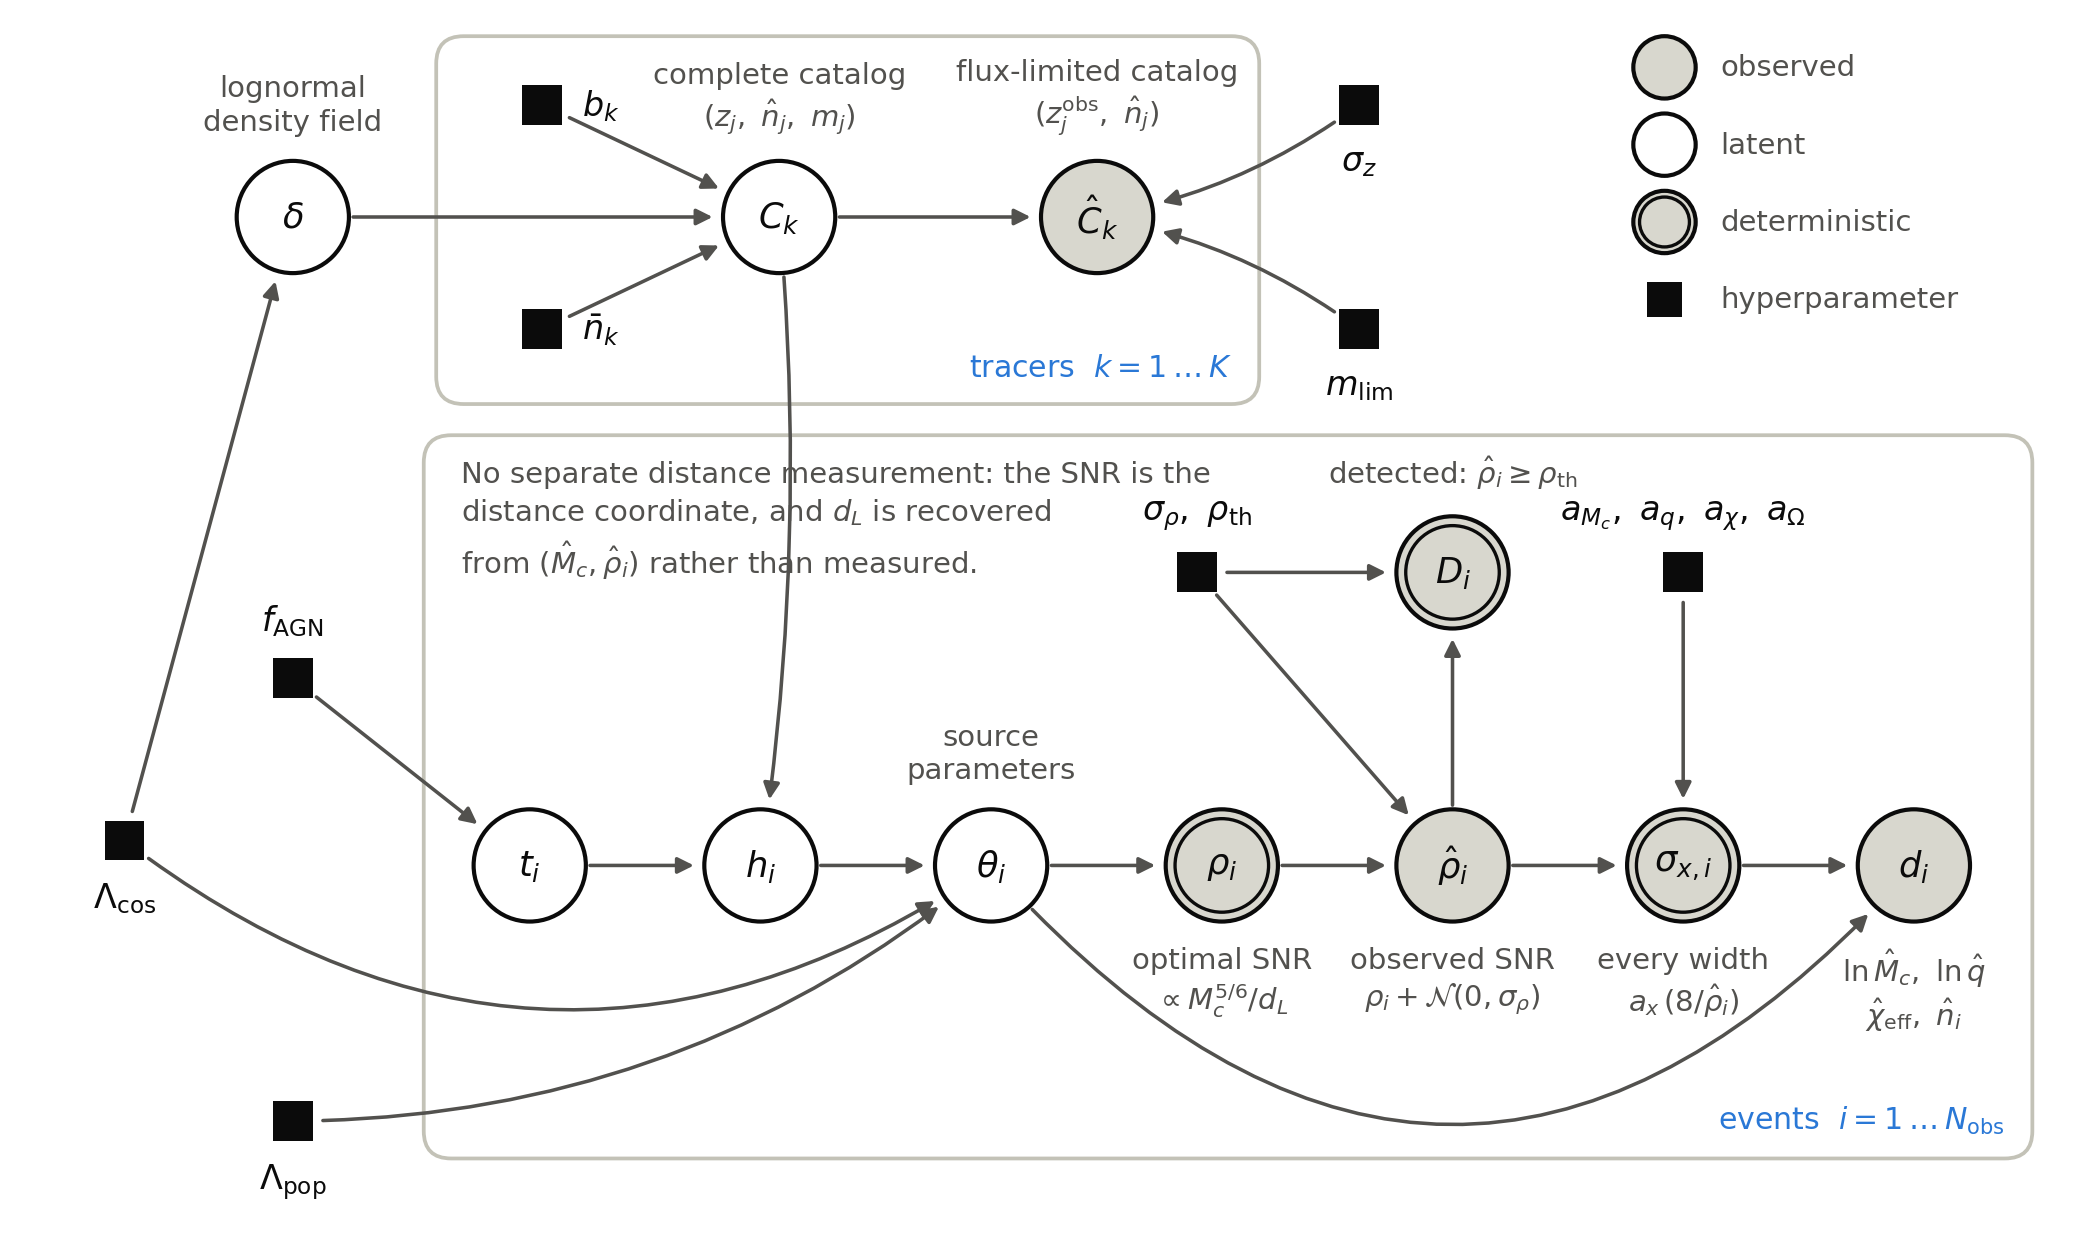
\includegraphics[width=\textwidth]{figures/fig_pgm.pdf}
\caption{The generative model of \S\ref{sec:data}. Shaded nodes are observed,
open nodes are latent, small filled squares are fixed hyperparameters, and
double-ringed nodes are deterministic functions of their parents. The cosmology
$\Lambda_{\rm cos}$ fixes the shell geometry and the matter power spectrum,
from which one lognormal density field $\delta$ is drawn. The tracer plate
($k = 1 \dots K$) samples that single field twice, each tracer with its own
linear bias $b_k$ and mean comoving density $\bar{n}_k$, into a complete
catalog $C_k$ of sky positions, photometric redshifts and magnitudes; the flux
limit $m_{\rm lim}$ thins $C_k$ into the observed catalog $\hat{C}_k$, the only
version the incomplete analyses see. The event plate ($i = 1 \dots \Nobs$)
draws a host-population label $t_i$ with probability \fagn, a host $h_i$ from
that population's \emph{complete} catalog (mergers occur whether or not a
survey catalogued the host), and source parameters $\theta_i$ from the fixed
population $\Lambda_{\rm pop}$. The source is measured once: the observed
amplitude $\rho_{{\rm obs},i}$ carries the measurement noise. Everything
downstream is a function of observed data, never of the latent source: the
detection indicator $D_i = \Theta(\rho_{{\rm obs},i} - \rho_{\rm th})$, every
measurement width, the observed direction $\hat{n}_i^{\rm obs}$, and the
derived luminosity distance. The
inference of \S\ref{sec:methods} conditions on the shaded nodes and infers
$(\Hz, \fagn)$.
\label{fig:pgm}}
\end{figure*}

\subsection{Two tracers of one density field}
\label{sec:data:field}

The background cosmology is flat $\Lambda$CDM with $\Hz = \HzeroTruth$~\kmsmpc,
$\Omega_{m,0} = \OmZeroTruth$ and $\Omega_{b,0} = \ObZeroTruth$
\citep{Planck2015}, and the nonlinear matter power spectrum is computed with
\textsc{camb} \citep{Lewis2000}. The light cone is divided into \FieldNshell\
shells of comoving thickness \FieldShellDx~Mpc out to $z = \FieldZmax$, each
with a linear radial window; projecting the matter power spectrum onto those
windows gives the shell--shell angular spectra, from which \textsc{glass}
\citep{Tessore2023} draws one realisation of a set of lognormal fields on a
HEALPix grid with $N_{\rm side} = \FieldNside$ and $\ell_{\rm max} =
\FieldLmax$. Lognormal rather than Gaussian fields matter because the sparse
tracer lives in the high-density tail.

Both tracers are sampled from that same realisation. The expected count of
tracer $k$ in pixel $p$ of shell $s$ is
\begin{equation}
  \lambda_{k,s,p} = \frac{\bar{n}_k V_{s}}{N_{\rm pix}}\,
     \max\!\left[\, 1 + b_k\, \delta_s(p),\; 0 \,\right],
  \label{eq:poisson}
\end{equation}
with $V_s$ the shell's comoving volume, and the realised count is an
independent Poisson draw; each object is placed uniformly within its pixel and
given a redshift drawn $\propto W_s(z)\,\dd V_c/\dd z$, which makes the comoving
number density constant.

The two number densities are anchored to the literature. For the galaxies we
take $\bar{n}_{\rm gal} = \NGal$~Mpc$^{-3}$, the density of the bright end of
the $B$-band Schechter function used to characterise the GLADE catalogs
($\phi^* = \PhiStar\,h^3$~Mpc$^{-3}$ with $h = 0.7$,
$\alpha = \SchechterAlpha$,
$M_B^* = \MagBStar$; \citealt{Dalya2018, Dalya2022}); on that luminosity
function the cut corresponds to $L > \LumCut\,L^*$, or
$M_B < \MagBLimit$. For the AGN we take $\bar{n}_{\rm AGN} = \NAgn$~Mpc$^{-3}$,
the space density of the luminous class $\log_{10} L_X(2$--$10\,{\rm keV})
\gtrsim 43.7$ from the integrated Swift-BAT/BASS X-ray luminosity function
\citep{Ananna2022}. The ratio of the two is \DensityRatioTarget. The linear
biases are $b_{\rm gal} = \BiasGal$ and $b_{\rm AGN} = \BiasAgn$, a contrast of
\BiasRatio.

The realised catalogs hold \CatNgal\ galaxies and \CatNagn\ AGN, with a
comoving number-density ratio of \DensityRatio. Cross-correlating the two
catalogs recovers a bias ratio of \BiasRatioMeas, within $2\sigma$ (1.1 per
cent) of the input \BiasRatio, so the clustering contrast that
Equation~(\ref{eq:mixture}) is asked to detect survives the resolution of the
field essentially undegraded.

Every object carries an absolute magnitude drawn from the same Schechter
function, converted to an apparent magnitude through the distance modulus with
no $K$-correction and no luminosity evolution. AGN inherit the luminosity
function of their host galaxies, so a single flux limit thins both catalogs
through the same completeness function and survey depth remains one axis rather
than two.

Catalogued redshifts are photometric. The observed redshift of every object is
scattered about the true one, $z_{\rm obs} = z + \mathcal{N}(0,
\epsilon_z(1+z))$ with $\epsilon_z = \CatDzScale$, the analysis sees only
$z_{\rm obs}$, and the per-object uncertainty the catalog declares matches the
scatter actually present (the normalised residuals have unit variance in both
catalogs). Mergers occur at the true redshift; the survey just does not know
it exactly.

The catalogs extend to $z = \FieldZmax$. This is a requirement rather than a
choice: the events reach $z = \EvHorizonZ$, and no posterior sample corresponds
to a redshift above $z = \PeZmax$ anywhere in the analysed range of \Hz, so the
catalogs' support extends well beyond the redshifts the gravitational-wave data
can reach and the edge of the catalog is never a lever on the inference.

\subsection{The gravitational-wave events}
\label{sec:data:events}

Events are placed on the complete catalogs, before any survey selection.

Each event is assigned a host population with probability \fagn, then a host
drawn uniformly from that population's catalog with an acceptance
$\propto (1+z)^{\gamma-1}$, so the merger redshift distribution is
$p(z) \propto (\dd V_c/\dd z)(1+z)^{\gamma-1}$ with $\gamma = \PopGamma$. The
event's redshift and sky position are its host's. Masses and effective spin are
drawn from a fixed power-law-plus-peak population independent of the host and
of the cosmology \citep{GWTC3Pop2023}, with $\alpha = \PopAlpha$,
$m_{\min} = \PopMmin\,\Msun$, $m_{\max} = \PopMmax\,\Msun$, taper widths
$\PopDmMin$ and $\PopDmMax\,\Msun$, peak weight $\PopPeakFrac$ at
$\mu = \PopPeakMu\,\Msun$ with $\sigma = \PopPeakSigma\,\Msun$, pairing index
$\beta = \PopBeta$, and $\chi \sim \mathcal{N}(0, \PopChiSigma^2)$. The input
AGN-hosted fraction is $\fagn = \EvFagn$, and events are drawn until
$\Nobs = \EvNobs$ are detected.

Each source is measured once, and that single measurement is the event. A single scalar
stands in for the network signal-to-noise ratio; its noise-free value depends
only on the detector-frame chirp mass and the luminosity distance,
\begin{equation}
  \rho_{\rm opt}\!\left(\mathcal{M}^{\rm det}, d_L\right) = \rho_{\rm ref}
     \left( \frac{\mathcal{M}^{\rm det}}{30\,\Msun} \right)^{5/6}
     \left( \frac{1\,{\rm Gpc}}{d_L} \right),
  \label{eq:snr}
\end{equation}
the inspiral scaling with the antenna response left out, with
$\rho_{\rm ref} = \EvSnrRef$ set so that the detected fraction matches a
calculation that includes the response. What is observed is this amplitude
plus its measurement noise,
$\rho_{\rm obs} = \rho_{\rm opt} + n$, $n \sim \mathcal{N}(0, \EvSigmaRho)$,
and an event is detected when $\rho_{\rm obs} \geq \EvSnrThresh$
\citep{FishbachHolzFarr2018, Farah2023}. Detection is therefore a threshold on
observed data, not on the source: Equation~(\ref{eq:zi}) is a density over the
observed data and $\mu$ normalises it over the detectable region, so the pair
is a correctly normalised density for detected events only if detection is a
property of the data themselves. \EvMalmquist\ per cent of the detected events
have a noise-free amplitude below threshold, the Malmquist scatter that only a
cut in data space produces.

Every measurement error follows the same rule: its width is a function of the
observed amplitude, never of the latent source. The detector-frame chirp mass,
mass ratio and effective spin are measured with
\begin{equation}
\begin{gathered}
  \sigma_{\ln \mathcal{M}} = \EvAmc\,\frac{\EvWidthRefSnr}{\rho_{\rm obs}},
  \qquad
  \sigma_{\ln q} = \EvAq\,\frac{\EvWidthRefSnr}{\rho_{\rm obs}},\\
  \sigma_{\chi} = \EvAchi\,\frac{\EvWidthRefSnr}{\rho_{\rm obs}},
\end{gathered}
  \label{eq:widths}
\end{equation}
the widths used to build mock catalogs for gravitational-wave population
studies \citep{FishbachHolzFarr2018, Farah2023}, and the observed sky position
is scattered about the host's with
$\sigma_{\rm ang} = \mathrm{clip}\!\left(
\EvSkyCoefEff^\circ/\rho_{\rm obs},\, \EvSkyMin^\circ,\, \EvSkyMax^\circ
\right)$, the $1/\rho$ scaling of timing triangulation \citep{Fairhurst2009};
the realised widths span \EvSkyMinReal--$\EvSkyMaxReal^\circ$. A width
computed from the true parameters instead would carry distance information
that the fixed-width posterior handed to the likelihood cannot represent.

There is no separate distance measurement. Given the observed chirp mass, the
observed amplitude fixes the distance by inverting Equation~(\ref{eq:snr}), so
the signal-to-noise ratio is the distance observable, with an effective width
$\sigma_{\ln d_L} = \EvSigmaLnDlCoef/\rho_{\rm obs}$: \EvSigmaLnDlThresh\
per cent at the detection threshold, with a median of \EvSigmaLnDlMedian\ in
$\ln d_L$ over the detected sample. Treating an independently measured
distance as a second datum alongside the amplitude would leave a
source-dependent factor in the likelihood that the inference has no parameter
for.

The event's posterior samples are exact. With flat priors on
$(\ln \mathcal{M}^{\rm det}, \ln q, \rho, \chi_{\rm eff}, \alpha, \delta)$,
the posterior conditioned on the observed values above is a product of known
one-dimensional distributions, and we draw \EvNsamp\ samples from it directly,
mapping the prior exactly into the $(m_1^{\rm det}, q, d_L, \chi_{\rm eff})$
basis the inference uses. Physical ranges ($q \leq 1$, $\rho > 0$,
$|\chi_{\rm eff}| \leq 1$) are imposed on the prior, never on the observed
values: truncating the data censors the likelihood, while truncating the
prior is exact. Sample clouds centred on the true parameters, by contrast,
would be mislabelled as flat-prior posteriors and would bias the distance
scale at order $\sigma_{\ln d_L}^2$.

The detected set contains \EvNhostGal\ galaxy-hosted and \EvNhostAgn\
AGN-hosted events, a realised fraction of \EvFagnReal\ against the input
probability of \EvFagn. It reaches $z = \EvHorizonZ$ with a median of
$z = \EvZmedian$; \EvNdetTotal\ of \EvNproposed\ proposed sources pass the
threshold (\EvDetFrac\ per cent), and the first \EvNobs\ constitute the
sample. The AGN-hosted events occupy \EvNuniqueAgn\ distinct AGN, with at most
\EvMaxPerAgn\ events sharing a host, so the sparse catalog is not carrying the
measurement through a handful of repeated hosts.

\subsection{Flux-limited catalogs}
\label{sec:data:survey}

Incomplete catalogs are produced by applying an apparent-magnitude limit
$m_j < m_{\rm lim}$ to the complete catalogs, with the same limit applied to
both tracers and the events left untouched. We use \MagLimN\ limits from
$m_{\rm lim} = \MagLimDeep$ to \MagLimShallow\ in steps of \MagLimStep\ mag.
Within the volume the events occupy, the fraction of galaxies catalogued is
\CompMTwentyOne\ per cent at the deepest limit and falls to \CompMTwenty,
\CompMNineteen\ and \CompMEighteen\ per cent at the shallower three, and the
AGN fractions differ from them by at most \CompAgnMaxDev\ percentage points.

The limit is isotropic and there is no explicit redshift cut. Both matter for
what is being measured: an anisotropic completeness modelled as isotropic by
Equation~(\ref{eq:completeness}) would imprint a sky-density contrast between
what the analysis expects and what it sees, which is the same contrast that
identifies \fagn; and letting $C_k(z)$ follow from the flux limit acting on the
luminosity function gives it the smoothly declining shape a flux-limited survey
has rather than one chosen for convenience.

The catalogs are pixelated at $N_{\rm side} = \SurveyNside$
(\SurveyNpix\ pixels) into the form Equation~(\ref{eq:pcat}) consumes, each
object entering at its observed redshift with its declared photometric
uncertainty as the kernel width, $\sigma_j = \epsilon_z(1 + z_{{\rm obs},j})$. At
this resolution the complete AGN catalog occupies every pixel, with up to
\AgnPerPix\ objects in one; at the shallowest limit \AgnEmptyPixShallow\ per
cent of pixels contain no AGN at all, and the emptiness of the sparse catalog
becomes part of the information: an AGN-hosted event cannot have come from a
pixel that holds no AGN, except through the out-of-catalog term of
\S\ref{sec:methods:completion}.

The selection function at every depth is estimated from the same
\InjNdrawMain\ injections, drawn against the complete catalogs from the
three-component mixture of \S\ref{sec:methods:selection} with weights
$\InjWeightPop$, $\InjWeightUni$ and $\InjWeightAgn$, and cross-checked
against \InjNdrawCross\ injections drawn from the population and the comoving
volume alone.
